% ==================///==================///==================///
% ==================/// LATEX'S STUFF
% ==================///==================///==================///

\documentclass[hungarian]{beamer}
\usepackage[T1]{fontenc}
\usepackage{babel}
\usepackage{graphicx}
\usepackage{hyperref}
\usepackage{stuki}

\usepackage{soul}

\usepackage{amsfonts,amsmath,oldgerm}
\usetheme{_statale}
\usefonttheme[onlymath]{serif}

\newcommand{\testcolor}[1]{\colorbox{#1}{\textcolor{#1}{test}}~\texttt{#1}}
\newcommand{\hrefcol}[2]{\textcolor{cyan}{\href{#1}{#2}}}
\titlebackground*{assets/background}

\newcommand{\Ord}{\mathcal{O}}


% ==================///==================///==================///
% ==================/// SPLASH PAGE
% ==================///==================///==================///

\title{Algoritmusok I.}
\newcommand{\longauthor}{3. gyakorlat}
\author{Sipos Ágoston}
\newcommand{\correspondingauthor}{John Doe}
\newcommand{\email}{siposagoston@inf.elte.hu}
\renewcommand{\insertdate}{2026. szeptember 23.}

% ==================///==================///==================///
% ==================/// START PRESENTATION
% ==================///==================///==================///

\begin{document}
\maketitle

\section{Sor}

\begin{frame}{Sor}

Nagyon hasonló a veremhez, analóg műveletek, annyi a különbség, hogy az új elemet a sor végére rakjuk; tehát az van a sor elején, ami legkorábban került be.

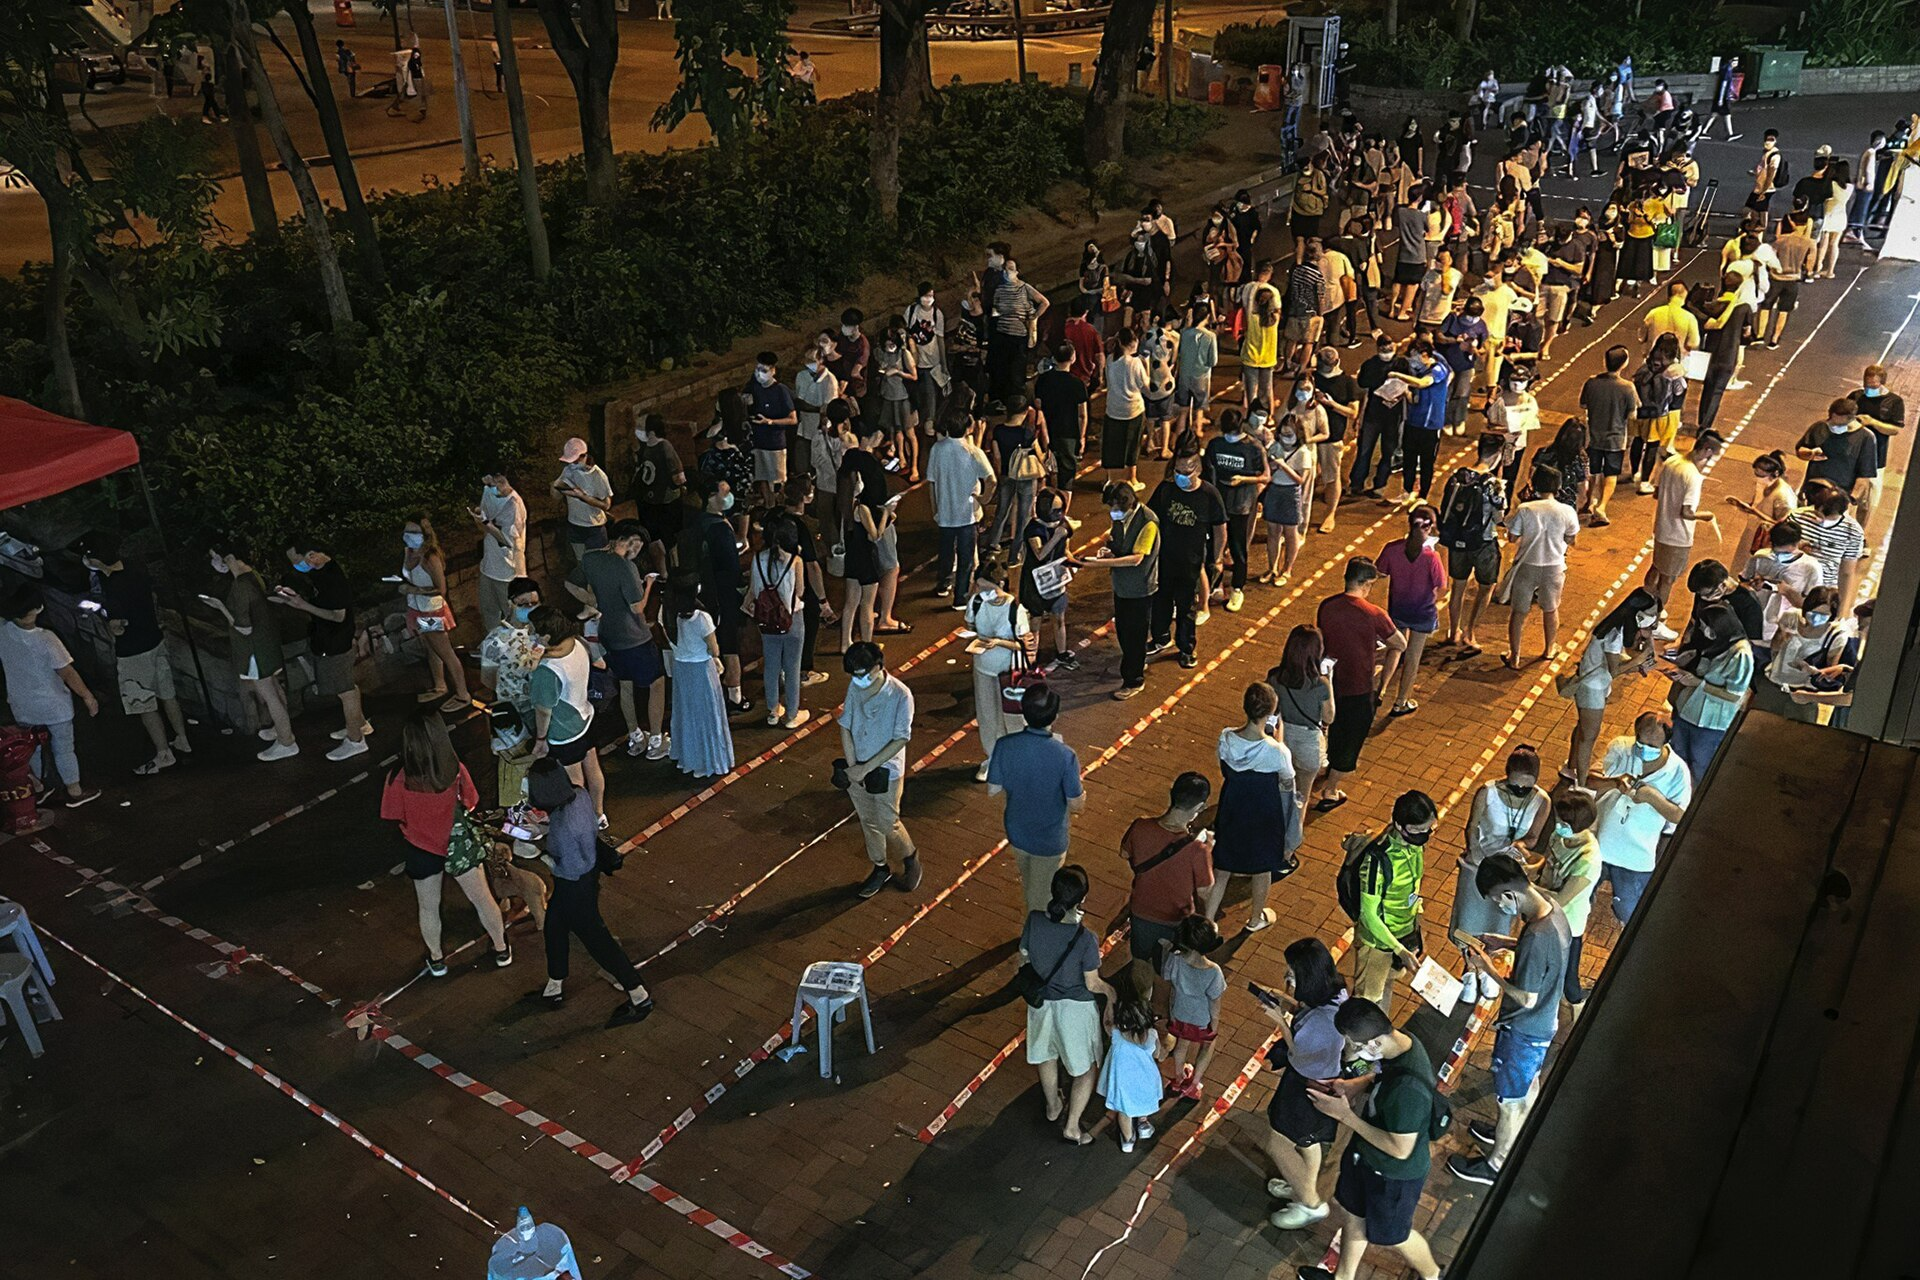
\includegraphics[width=0.5\linewidth]{assets/hongkong.png}

\end{frame}

\begin{frame}{Sorműveletek}

Queue() -- létrehoz egy üres sort

add(x : T) -- az x elemet a sor végére teszi

rem(): T -- a sor legelső elemét eltávolítja, és visszaadja

first(): T -- a sor legelső elemét visszaadja

isEmpty(): $\mathbb{B}$ -- visszaadja, hogy van-e elem a sorban


Egyelőre maradjunk ezen az absztrakciós szinten, ne vizsgáljuk hogyan implementálnánk.
    
\end{frame}

\begin{frame}{,,Dadogó'' szavak problémája}

Bemenetről érkezik egy szöveg és el kell dönteni, hogy a bemeneti szöveg ,,dadogós''-e vagy sem.

Példa: ``aa'', ``almaalma'', <> (üres szöveg is dadogósnak tekinthető)

Ötlet:

\begin{itemize}
    \item Olvassuk be a szöveget egy sorba.
    \item Ha a hossz páratlan, akkor nem ,,dadogós''.
    \item Ha páros, az egyik felét másoljuk egy másik sorba, majd hasonlítsuk össze.
\end{itemize}

\end{frame}

\begin{frame}[t]{,,Dadogó'' szavak problémája}

Bemenetről érkezik egy szöveg és el kell dönteni, hogy a bemeneti szöveg ,,dadogós''-e vagy sem.

\end{frame}

\begin{frame}[t]{Pascal-háromszög kiszámítása}

\[
\begin{array}{c}
       1 \\
     1 \quad 1 \\
   1 \quad 2 \quad 1 \\
 1 \quad 3 \quad 3 \quad 1
\end{array}
\]

Adott $k$ esetén számítsuk ki a $k$. sort.

Ne használjuk a direkt képletet: $\dfrac{k!}{i!\cdot(k-i)!}$

Dolgozzon az algoritmus sorról sorra, és használja ki, hogy minden szám a felette levő kettő összege.

\end{frame}

\begin{frame}[t]{Pascal-háromszög kiszámítása}

Bemenet: $k \in \mathbb{N}$ (az ennyiedik sort akarjuk kiszámítani)

\end{frame}

\section{Láncolt lista}

\begin{frame}{Láncolt lista}

A lista minden eleme tartalmaz egy mutatót a következő elemre.

Fajtái:
\begin{itemize}
    \item Egyszerű,egyirányú láncolt lista (S1L)
    \item Fejelemes egyirányú láncolt lista (H1L)
    \item Ciklikus egyirányú lista (C1L)
    \item Egyszerű, kétirányú lista (S2L)
    \item Ciklikus kétirányú lista (C2L) fejelemmel
\end{itemize}

\end{frame}

\begin{frame}{Egyszerű, egyirányú láncolt lista (S1L)}

\begin{figure}
    \centering
    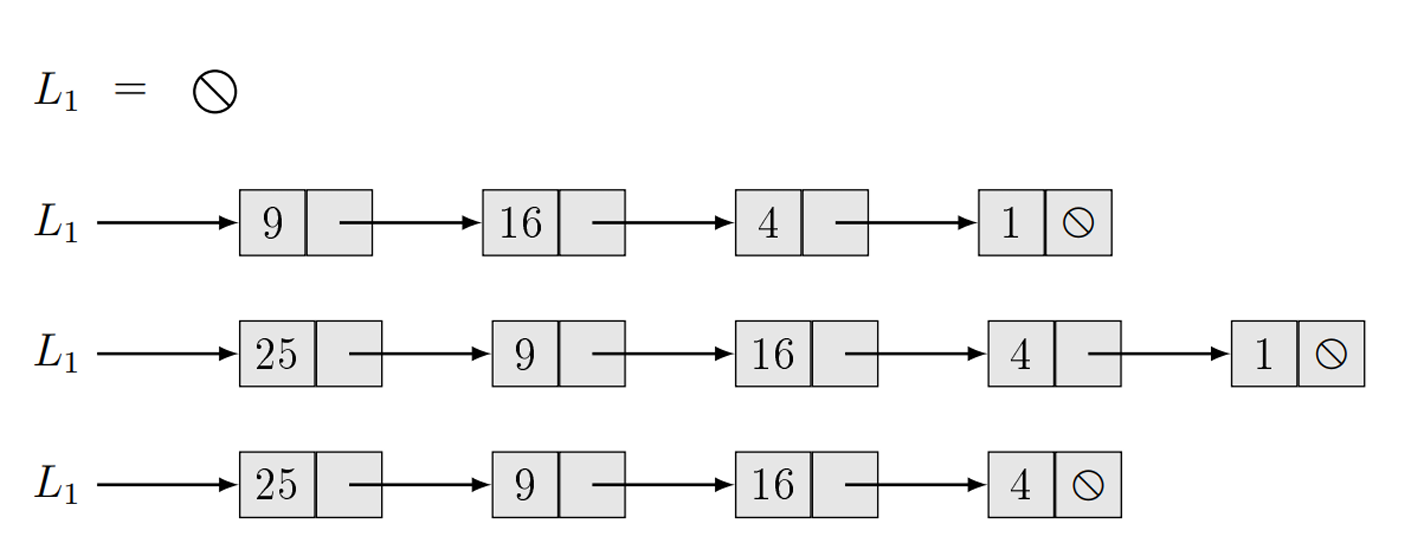
\includegraphics[width=0.8\linewidth]{assets/linked.png}
\end{figure}

Minden listaelem rendelkezik a) a saját adatával; b) egy mutatóval a következő elemre.

A lista utolsó elemének mutatója NULL

L maga egy mutató; ha a lista üres, akkor L=NULL

\end{frame}

\begin{frame}{Láncolt lista -- jelölések}

\begin{figure}
    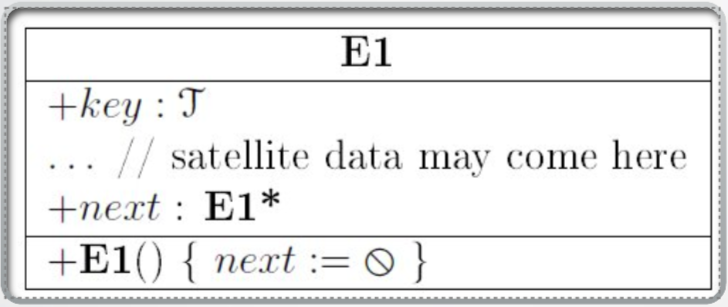
\includegraphics[width=0.4\linewidth]{assets/element.png}
\end{figure}


\begin{columns}
\begin{column}{0.6\linewidth}

L lista esetén (L típusa E1*)

\begin{itemize}
    \item L: az első elem címe; *L az első elem
    \item L->key: az első elem kulcsértéke (vagy (*L).key)
    \item L->next: a második elem címe
    \item L->next->key: a második elem kulcsértéke
    \item \dots
\end{itemize}

\end{column}
\begin{column}{0.4\linewidth}
    Listaelem létrehozása: q = new E1

    Ekkor q-ban E1 \textit{címe} van
\end{column}
\end{columns}

\end{frame}


\begin{frame}[t]{Egyszerű, egyirányú láncolt lista (S1L) -- iterálás}

\only<1>{1. Írjuk ki a lista összes kulcsát!}

\only<2>{2. Keressük meg az adott kulcsú elem címét!}

Bemenet: L: E1*\only<2>{, k: $\mathcal{T}$}

\end{frame}

\begin{frame}{Egyszerű, egyirányú láncolt lista (S1L) -- beszúrás}

\begin{columns}
\begin{column}{0.4\linewidth}
Szúrjunk be egy k kulcsú elemet a listába, adott helyre.

Több eset lehetséges:
\begin{itemize}
    \item \only<1>{\textbf{A lista elejére}}\only<2-4>{A lista elejére}
    \only<2-4>{\item \only<2>{\textbf}{A lista belsejébe}}
    \only<3-4>{\item \only<3>{\textbf}{A lista végére}}
    \only<4>{\item \only<4>{\textbf}{Üres listába}}
\end{itemize}

\end{column}
\begin{column}{0.4\linewidth}

\only<1>{
\setlength{\stukiwidth}{4cm}
\begin{stukibox}
\stm*{q = new E1}
\stm*{q->key = k}
\stm*{q->next = L}
\stm*{L = q}
\end{stukibox}
}
\only<2>{
p az elem címe ami mögé beszúrjuk (ef. p->next != NULL)
\setlength{\stukiwidth}{4cm}
\begin{stukibox}
\stm*{q = new E1}
\stm*{q->key = k}
\stm*{q->next = p->next}
\stm*{p->next = q}
\end{stukibox}
}
\only<3>{
p az utolsó elem címe ami mögé beszúrjuk (ef. p->next = NULL)
\setlength{\stukiwidth}{4cm}
\begin{stukibox}
\stm*{q = new E1}
\stm*{q->key = k}
\stm*{q->next = NULL}
\stm*{p->next = q}
\end{stukibox}
}
\only<4>{
\setlength{\stukiwidth}{4cm}
\begin{stukibox}
\stm*{q = new E1}
\stm*{q->key = k}
\stm*{q->next = NULL}
\stm*{L = q}
\end{stukibox}
}

\end{column}

\end{columns}
\end{frame}

\begin{frame}[t]{Egyszerű, egyirányú láncolt lista (S1L) -- törlés}

Vegyünk ki egy (p című) elemet a listából! Ez azt jelenti, hogy ezután az előtte levő elem az utána levő elemre mutat.

Most is számít: első elemet töröljük (L=p), vagy nem.

\end{frame}

\section{Feladatok}

\begin{frame}[t]{Lista megfordítása}

Legyen L egy S1L. Fordítsuk meg az elemek sorrendjét. Ne végezzünk másolásokat (azaz csak mutatókat állítsunk, ne konstruáljunk új listaelemeket).

\only<1>{

Bemenet: L→egy→kettő→három→négy

Kimenet: L→négy→három→kettő→egy
}

\only<2>{Ötlet: végigiterálunk a listán, és sorban beszúrjuk az elemeit egy új üres lista elejére.}

\end{frame}

\begin{frame}{Prímszitálás}

Eratoszthenész (Kr.e. 3. század)

Határozzuk meg a prímszámokat 1-től n-ig.

Ötlet: tegyünk minden számot egy listába. Majd induljunk el 2-től, és minden többszörösét vegyük ki. Ismételjük 3-ra, stb. Ami marad, azok a prímszámok.

\vspace{5mm}

\begin{tabular}{|c|c|c|c|c|c|c|c|c|}
    \hline
    2 & 3 & 4 & 5 & 6 & 7 & 8 & 9 & 10 \\
    \hline
\end{tabular}

\begin{tabular}{|c|c|c|c|c|c|c|c|c|}
    \hline
    2 & 3 & \st{4} & 5 & \st{6} & 7 & \st{8} & 9 & \st{10} \\
    \hline
\end{tabular}

\begin{tabular}{|c|c|c|c|c|c|c|c|c|}
    \hline
    \textbf{2} & \textbf{3} & \st{4} & \textbf{5} & \st{6} & \textbf{7} & \st{8} & \st{9} & \st{10} \\
    \hline
\end{tabular}
    
\end{frame}

\begin{frame}{Prímszitálás -- algoritmus}

\end{frame}

\end{document}
